%%%%%%%%%%%%%%%%%%%%%%%%%%%%%%%%%%%%%%%%%
% Beamer Presentation
% LaTeX Template
% Version 1.0 (10/11/12)
%
% This template has been downloaded from:
% http://www.LaTeXTemplates.com
%
% License:
% CC BY-NC-SA 3.0 (http://creativecommons.org/licenses/by-nc-sa/3.0/)
%
%%%%%%%%%%%%%%%%%%%%%%%%%%%%%%%%%%%%%%%%%

%----------------------------------------------------------------------------------------
%	PACKAGES AND THEMES
%----------------------------------------------------------------------------------------
\documentclass{beamer}

\mode<presentation> {

% The Beamer class comes with a number of default slide themes
% which change the colors and layouts of slides. Below this is a list
% of all the themes, uncomment each in turn to see what they look like.

%\usetheme{default}
%\usetheme{AnnArbor}
%\usetheme{Antibes}
%\usetheme{Bergen}
%\usetheme{Berkeley}
%\usetheme{Berlin}
%\usetheme{Boadilla}
%\usetheme{CambridgeUS}
%\usetheme{Copenhagen}
%\usetheme{Darmstadt}
%\usetheme{Dresden}
%\usetheme{Frankfurt}
%\usetheme{Goettingen}
%\usetheme{Hannover}
%\usetheme{Ilmenau}
%\usetheme{JuanLesPins}
%\usetheme{Luebeck}
\usetheme{Madrid}
%\usetheme{Malmoe}
%\usetheme{Marburg}
%\usetheme{Montpellier}
%\usetheme{PaloAlto}
%\usetheme{Pittsburgh}
%\usetheme{Rochester}
%\usetheme{Singapore}
%\usetheme{Szeged}
%\usetheme{Warsaw}

% As well as themes, the Beamer class has a number of color themes
% for any slide theme. Uncomment each of these in turn to see how it
% changes the colors of your current slide theme.

%\usecolortheme{albatross}
%\usecolortheme{beaver}
%\usecolortheme{beetle}
%\usecolortheme{crane}
%\usecolortheme{dolphin}
%\usecolortheme{dove}
%\usecolortheme{fly}
%\usecolortheme{lily}
%\usecolortheme{orchid}
%\usecolortheme{rose}
%\usecolortheme{seagull}
%\usecolortheme{seahorse}
%\usecolortheme{whale}
%\usecolortheme{wolverine}

%\setbeamertemplate{footline} % To remove the footer line in all slides uncomment this line
%\setbeamertemplate{footline}[page number] % To replace the footer line in all slides with a simple slide count uncomment this line

%\setbeamertemplate{navigation symbols}{} % To remove the navigation symbols from the bottom of all slides uncomment this line
}
%----------------------------------------------------------------------------------------
\usepackage{graphicx} % Allows including images
\usepackage{booktabs} % Allows the use of \toprule, \midrule and \bottomrule in tables
\usepackage{subfigure}
\setbeamerfont{caption}{size=\scriptsize}
\usepackage{hyperref}
\usepackage{listings}
%----------------------------------------------------------------------------------------
%	TITLE PAGE
%----------------------------------------------------------------------------------------
\title[]{ROS Build/Debug Utilities and Launch-Files} % The short title appears at the bottom of every slide, the full title is only on the title page
%----------------------------------------------------------------------------------------
\author{ARRA / AR2A} % Your name
\institute % Your institution as it will appear on the bottom of every slide, may be shorthand to save space
{
\textbf{A}dvancements for \textbf{R}obotics in \textbf{R}escue \textbf{A}pplications
}
\date{\today} % Date, can be changed to a custom date
%----------------------------------------------------------------------------------------
\AtBeginSection{\frame{\sectionpage}}
%----------------------------------------------------------------------------------------
\begin{document}
%----------------------------------------------------------------------------------------
\begin{frame}
\titlepage % Print the title page as the first slide
\end{frame}
%----------------------------------------------------------------------------------------
\begin{frame}
\frametitle{Overview} % Table of contents slide, comment this block out to remove it
\tableofcontents % Throughout your presentation, if you choose to use \section{} and \subsection{} commands, these will automatically be printed on this slide as an overview of your presentation
\end{frame}
%----------------------------------------------------------------------------------------
%	PRESENTATION SLIDES
%----------------------------------------------------------------------------------------
\section{Debug Utilities}
%----------------------------------------------------------------------------------------
\begin{frame}{Debug - Overview}
	\begin{large}\textbf{Interacting with and debugging running system:}\end{large}
	\begin{itemize}
		\item Topics: 							rostopic
		\item Services:							rosservice and rossrv
		\item Messages:							rosmsg
	\end{itemize}
\end{frame}
%----------------------------------------------------------------------------------------
\begin{frame}{Debug - rostopic}
The rostopic tool allows you to get information about ROS topics.
\newline
\newline
\begin{large}\textbf{Available sub-commands:}\end{large}
\begin{itemize}
	\item rostopic bw:     \textit{display bandwidth used by topic}
	\item rostopic echo:   \textit{print messages to screen}
	\item rostopic hz:     \textit{display publishing rate of topic}    
	\item rostopic list:   \textit{print information about active topics}
	\item rostopic pub:    \textit{publish data to topic}
	\item rostopic type:   \textit{print topic type}
\end{itemize}
\end{frame}
%----------------------------------------------------------------------------------------
\begin{frame}{rostopic - Example}
A given turtle demo was used for the following example.
\newline
The \textit{list} command prints information about the active topics on the screen.
\newline
\textbf{Command:} 

\lstinputlisting[frame=single, basicstyle=\footnotesize\ttfamily, language=C]{./listings/rostopic.txt}

\textbf{Output:}
\lstinputlisting[frame=single, basicstyle=\footnotesize\ttfamily, language=C]{./listings/rostopic_output.txt}

\end{frame}
%----------------------------------------------------------------------------------------
\begin{frame}{rostopic - Example}
The \textit{echo} command shows the messages from the topics on the screen.
\newline
\textbf{Command:} 
\lstinputlisting[frame=single, basicstyle=\footnotesize\ttfamily, language=C]{./listings/rostopic_echo.txt}
\textbf{Output:}
\lstinputlisting[frame=single, basicstyle=\footnotesize\ttfamily, language=C]{./listings/rostopic_echo_2.txt}
\end{frame}
%----------------------------------------------------------------------------------------
\begin{frame}{Debug - rosservice}
rosservice can easily attach to ROS's client/service framework with services. rosservice has many commands that can be used on topics, as shown below:
\newline
\newline
\begin{large}\textbf{Available sub-commands:}\end{large}
\begin{itemize}
	\item rosservice list:   \textit{ print information about active services}
	\item rosservice call:   \textit{call the service with the provided args}
	\item rosservice type:   \textit{print service type}    
	\item rosservice find:   \textit{find services by service type}
	\item rosservice uri:    \textit{ print service ROSRPC uri}
\end{itemize}
\end{frame}
%----------------------------------------------------------------------------------------
\begin{frame}{rosservice - Example}
A given turtle demo was used for the following example.
\newline
The \textit{list} command shows the services from the turtlesim node demo.
\textbf{Command:} 
\lstinputlisting[frame=single, basicstyle=\footnotesize\ttfamily, language=C]{./listings/rosservice_list.txt}

\textbf{Output:}
\lstinputlisting[frame=single, basicstyle=\footnotesize\ttfamily, language=C]{./listings/rosservice_list_2.txt}
\end{frame}
%----------------------------------------------------------------------------------------
\begin{frame}{rosservice - Example}
The \textit{type} command shows what type the service is.
\newline
\newline
\textbf{Command:} 
\lstinputlisting[frame=single, basicstyle=\footnotesize\ttfamily, language=C]{./listings/rosservice_clear.txt}
\textbf{Output:}
\lstinputlisting[frame=single, basicstyle=\footnotesize\ttfamily, language=C]{./listings/rosservice_clear_1.txt}
This service is empty, this means when the service call is made it takes no arguments (i.e. it sends no data when making a request and receives no data when receiving a response).
\end{frame}
%----------------------------------------------------------------------------------------
\begin{frame}{rosservice - Example}
The \textit{call} command perform the used service.
\textbf{Command:} 
\lstinputlisting[frame=single, basicstyle=\footnotesize\ttfamily, language=C]{./listings/rosservice_clear_2.txt}
There are no further arguments because the service is of type empty.
\newline
Otherwise the usage is:
\lstinputlisting[frame=single, basicstyle=\footnotesize\ttfamily, language=C]{./listings/rosservice_clear_3.txt}
This does what expected, it clears the background of the turtlesim\_node.
\begin{figure}[h]\centering
	\subfigure[Figure 1]{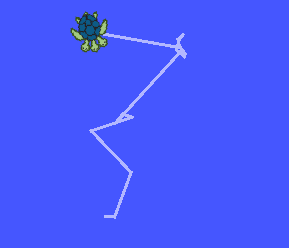
\includegraphics[width = 0.26\textwidth]{./images/turtle_line.png}}
	\subfigure[Figure 2]{
\includegraphics[width = 0.285\textwidth]{./images/turtle_clear.png}}
\end{figure}
\end{frame}
%----------------------------------------------------------------------------------------
\begin{frame}{Debug - rosmsg and rossrv}
	\textbf{rosmsg} contains two command-line tools:
	\begin{itemize}
		\item \textbf{rosmsg}
		\item \textbf{rossrv}
	\end{itemize}
	These are handy command-line tools that provide reference information for developers and also serve as a powerful introspection tool for learning more about data being transmitted in ROS.
\end{frame}
%----------------------------------------------------------------------------------------
\begin{frame}{Debug - rosmsg}
	\textbf{rosmsg} is a command-line tool for displaying information about ROS Message types.
	\newline
	\newline
	\begin{large}\textbf{Available sub-commands for rosmsg:}\end{large}
	\begin{itemize}
		\item rosmsg show: Show message description 
		\item rosmsg list: List all messages
		\item rosmsg md5: Display message md5sum
		\item rosmsg package: List messages in a package
		\item rosmsg packages: List packages that contain messages
	\end{itemize}
\end{frame}
%----------------------------------------------------------------------------------------
\begin{frame}{rosmsg - Example}
The \textit{type} command shows what type the service is.
\newline
\textbf{Command:} 
\lstinputlisting[frame=single, basicstyle=\footnotesize\ttfamily, language=C]{./listings/rosmsg_type.txt}

\textbf{Output:}
\lstinputlisting[frame=single, basicstyle=\footnotesize\ttfamily, language=C]{./listings/rosmsg_type_1.txt}
\end{frame}
%----------------------------------------------------------------------------------------
\begin{frame}{Debug - rossrv}
	\textbf{rossrv} is a command-line tool for displaying information about ROS Service types.
	\newline
	\newline
	\begin{large}\textbf{Available sub-commands for rossrv:}\end{large}
	\begin{itemize}
		\item rossrv show: Show service description
		\item rossrv list: List all services
		\item rossrv md5: Display service md5sum
		\item rossrv package: List services in a package
		\item rossrv packages: List packages that contain services
		
	\end{itemize}
\end{frame}
%----------------------------------------------------------------------------------------
\section{GUI development - rqt}
%----------------------------------------------------------------------------------------
\begin{frame}{Debug with rqt}
	\textbf{rqt} is a software framework of ROS that implements the various GUI tools in the form of plugins. \\ One can run all the existing GUI tools as dockable windows within rqt!
	\newline
	\newline
	There are also different opportunities to debug with rqt plugins. For example with the \textbf{Console} plugin under \textbf{Plugins/Logging} displays messages as seen in example 1 and 2.
\end{frame}
%----------------------------------------------------------------------------------------
\begin{frame}{rqt Example 1}
\begin{figure}[p]
	\centering
	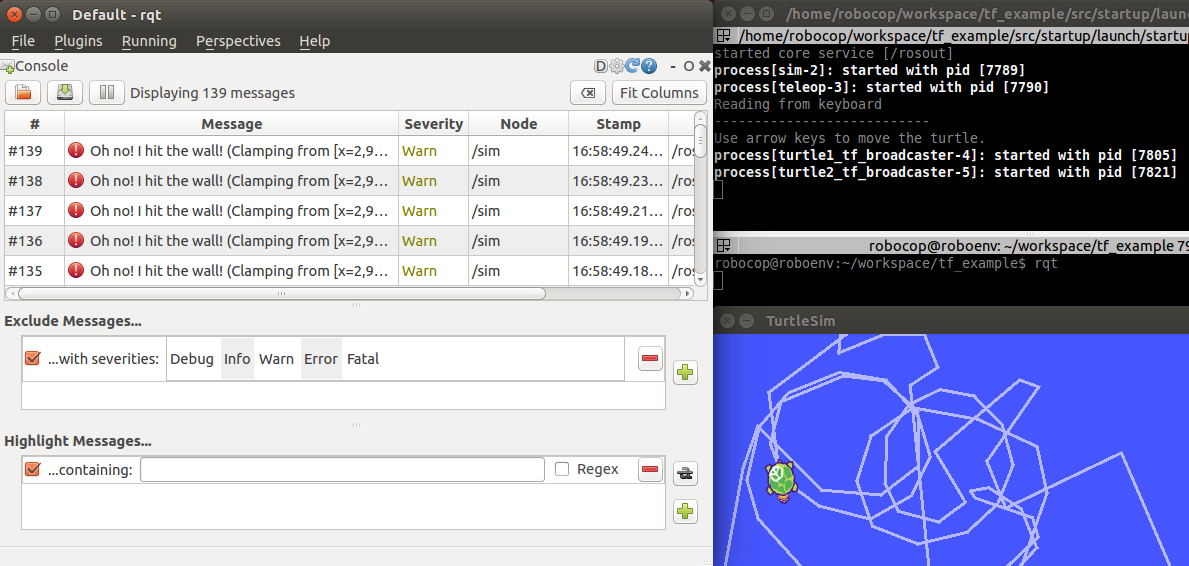
\includegraphics[width=1\textwidth]{./images/rqt.png}
	\caption{Read messages with rqt turtle demo.}
	\label{fig::rqt}
\end{figure}
\end{frame}
%----------------------------------------------------------------------------------------
\begin{frame}{rqt Example 2}
	\begin{figure}[p]
		\centering
		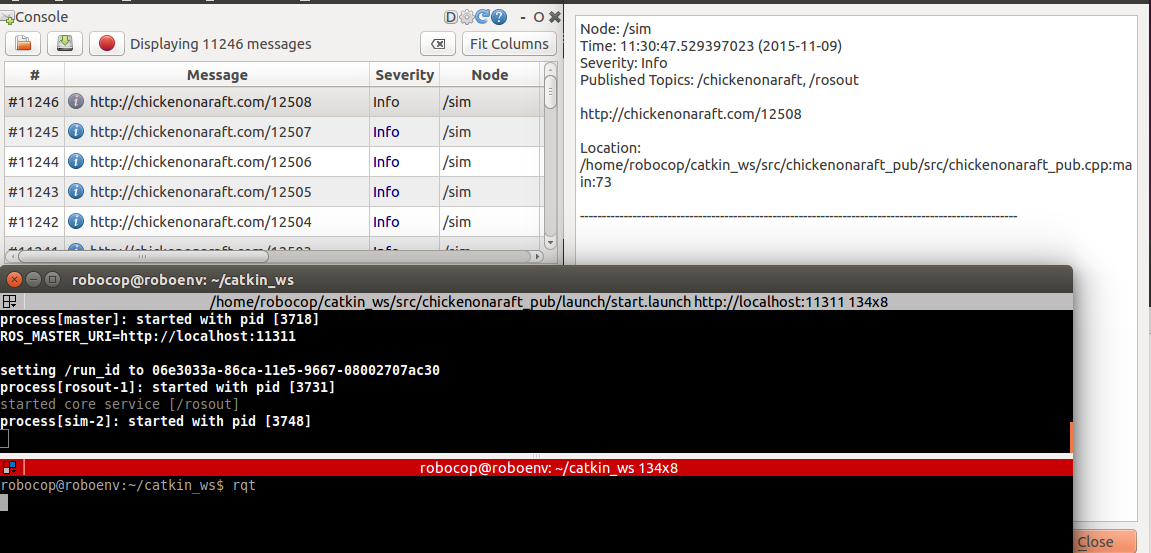
\includegraphics[width=1\textwidth]{./images/chickenrqt.png}
		\caption{Read messages with rqt from chicken demo.}
		\label{fig::rqt}
	\end{figure}
\end{frame}
%----------------------------------------------------------------------------------------
\section{Launch Files}
%----------------------------------------------------------------------------------------
\begin{frame}{Launch Files}
\begin{large}
	\textbf{roslaunch} \newline \newline
\end{large}
roslaunch is a tool for easily launching multiple ROS nodes locally and remotely via SSH, as well as setting parameters on the Parameter Server. \newline \newline
It takes in one or more XML configuration files (with the .launch extension) that specify the parameters to set and nodes to launch.
\end{frame}
%----------------------------------------------------------------------------------------
\begin{frame}{Launch Files}
	\begin{large}
		\textbf{Advantages:} \newline
	\end{large}
\begin{itemize}
	\item Starting implicitly the ROS "core", that's a collection of nodes and programs that are pre-requisites of a ROS-based system.
	\newline
	\item The launch file syntax itself is stable, and every effort will be made to provide backwards compatibility with new features. 
	\newline
	\item Option to set the necessary parameters for the single packages. 
\end{itemize}
\end{frame}
%----------------------------------------------------------------------------------------
\begin{frame}{Launch Files}
Many ROS packages come with "launch files", which can be runned with:

\lstinputlisting[frame=single, basicstyle=\footnotesize\ttfamily, language=C]{./listings/launch.txt}

These launch files usually bring up a set of nodes for the package that provide some aggregate functionality. 
\end{frame}
%----------------------------------------------------------------------------------------
\begin{frame}{Launch Files - Example 1}
\begin{large}
	\textbf{Launch-File from example learning\_tf} 
\end{large}
\lstinputlisting[frame=single, basicstyle=\footnotesize\ttfamily, language=C]{./listings/launch_2.txt}
\end{frame}
%----------------------------------------------------------------------------------------
\begin{frame}{Launch Files - Example 2}
	\begin{large}
		\textbf{Launch-File from example chickenonaraft} 
	\end{large}
\lstinputlisting[frame=single, basicstyle=\footnotesize\ttfamily, language=C]{./listings/launch_3.txt}
\end{frame}
%----------------------------------------------------------------------------------------
\begin{frame}{Launch Files}
	The stucture of the path is usually: \\
\lstinputlisting[frame=single, basicstyle=\footnotesize\ttfamily, language=C]{./listings/launch_4.txt}
	
	Large applications on a robot typically involve several interconnected nodes, each of which have many parameters. For this you can create a separately package only for the startup launch file:
\lstinputlisting[frame=single, basicstyle=\footnotesize\ttfamily, language=C]{./listings/launch_5.txt}
	For the startup package are no further dependencies necessary.
	
\end{frame}
%----------------------------------------------------------------------------------------
\begin{frame}{Launch Files}
In the separately package the launch file calls the other launch files:
\lstinputlisting[frame=single, basicstyle=\footnotesize\ttfamily, language=C]{./listings/launch_1.txt}
\end{frame}
%----------------------------------------------------------------------------------------
\begin{frame}
\Huge{\centerline{The End}}
\end{frame}
%----------------------------------------------------------------------------------------
\end{document} 
%----------------------------------------------------------------------------------------